\documentclass[aspectratio=169,10pt]{beamer}
\usetheme{Madrid}
\usecolortheme{seahorse}

\usepackage{amsmath}
\usepackage{amssymb}
\usepackage{amsfonts}
\usepackage{mathtools}
\usepackage{xcolor}
\usepackage{listings}
\usepackage{graphicx}
\usepackage{color}
\usepackage{hyperref}
\usepackage{bm}

\graphicspath{{figures/}}

% Define custom colors
\definecolor{codebg}{gray}{0.95}
\definecolor{codeframe}{gray}{0.7}

% Listings setup
\lstset{
    basicstyle=\ttfamily\scriptsize,
    commentstyle=\color{green!50!black}\itshape,
    keywordstyle=\color{blue},
    numberstyle=\tiny\color{gray},
    numbers=left,
    frame=single,
    framexleftmargin=0.8em,
    backgroundcolor=\color{codebg},
    rulecolor=\color{codeframe},
    breaklines=true,
    showstringspaces=false,
    captionpos=b
}

\setbeamertemplate{footline}[frame number]

\title{Chapter 6a: Degree Theory and Differential Calculus in Banach Spaces}
\subtitle{Pathak: Introduction to Nonlinear Analysis and Fixed Point Theory}
\author{Lecture Notes}
\date{\today}

\begin{document}

\frame{\titlepage}

\begin{frame}
\frametitle{Chapter Overview}
\begin{itemize}
    \item \textbf{Section 6.1:} The Topological Degree
    \begin{itemize}
        \item Axioms and definition in finite dimensions
        \item Brouwer degree theory
        \item Leray-Schauder degree for infinite dimensions
    \end{itemize}
    \vspace{0.3cm}
    \item \textbf{Section 6.2:} Degree Theory of Completely Continuous Vector Fields
    \begin{itemize}
        \item Extension to Banach spaces
        \item Homotopy properties and invariance
        \item Applications to operator equations and ODEs
    \end{itemize}
    \vspace{0.3cm}
    \item \textbf{Key Goals:}
    \begin{itemize}
        \item Extend fixed point theory to infinite dimensions
        \item Prove existence of solutions without explicit computation
        \item Study properties preserved under continuous deformations
    \end{itemize}
\end{itemize}
\end{frame}

% ============================================================================
% SECTION 6.1: THE TOPOLOGICAL DEGREE
% ============================================================================

\section{Section 6.1: The Topological Degree}

\begin{frame}
\frametitle{6.1.0: Historical Context and Motivation}
\begin{itemize}
    \item \textbf{Brouwer (1912):} Introduced the concept of local degree in $\mathbb{R}^n$
    \vspace{0.2cm}
    \item \textbf{Hadamard:} Developed theory and provided detailed discussion
    \vspace{0.2cm}
    \item \textbf{Brouwer:} Extended to large degree and proved many famous fixed point results
    \vspace{0.2cm}
    \item \textbf{Leray-Schauder:} Simple construction extending degree to infinite dimensions
    \vspace{0.2cm}
    \item \textbf{Applications:} Existence results for nonlinear operator equations without explicit solutions
\end{itemize}

\vspace{0.4cm}
\textbf{Central Question:}
For equation $f(x) = y$ where $f: \Omega \to \mathbb{R}^n$, can we determine number of solutions?
\end{frame}

\begin{frame}
\frametitle{6.1.1: Basic Concepts}

\textbf{Definition 6.1:} (Homotopy)
If $f_1, f_2: X \to Y$ are continuous maps, a \emph{homotopy} from $f_1$ to $f_2$ is a continuous map
$$H: [0,1] \times X \to Y \quad \text{such that} \quad H(0,x) = f_1(x), \quad H(1,x) = f_2(x)$$
Write $f_1 \simeq f_2$ if such a homotopy exists.

\vspace{0.3cm}
\textbf{Key Insight:} Homotopy formalizes the idea of continuous deformation.
\begin{center}
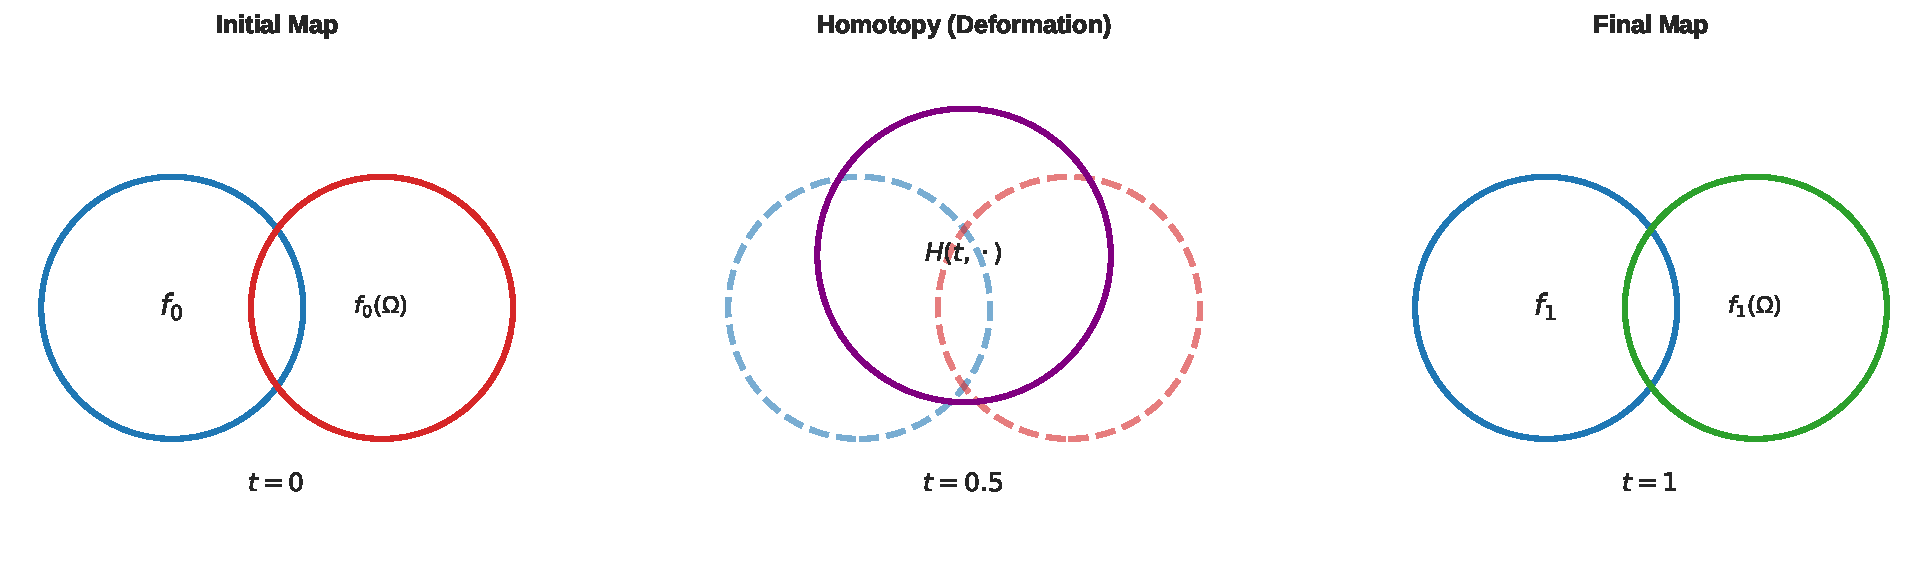
\includegraphics[width=0.8\textwidth]{homotopy_concept.pdf}
\end{center}
\end{frame}

\begin{frame}
\frametitle{6.1.1: Axioms of Brouwer Degree}

\textbf{Setup:} $\Omega \subseteq \mathbb{R}^n$ open and bounded, $f: \Omega \to \mathbb{R}^n$ continuous, $y \in \mathbb{R}^n$.

\vspace{0.3cm}
\textbf{Definition 6.2:} The degree $\deg(f, \Omega, y)$ is an integer assigned to each admissible triple $(f, \Omega, y)$ such that:

\begin{enumerate}
    \item \textbf{Existence:} $\deg(f, \Omega, y) \neq 0 \Rightarrow \exists x \in \Omega: f(x) = y$
    \vspace{0.2cm}
    \item \textbf{Homotopy Invariance:} If $H: [0,1] \times \Omega \to \mathbb{R}^n$ continuous with $H(t,x) \neq y$ on $\partial\Omega$ and all $t \in [0,1]$, then $\deg(H(t,\cdot), \Omega, y)$ is constant in $t$
    \vspace{0.2cm}
    \item \textbf{Normalization:} For identity map $I$ and open ball $\mathbb{B}$,
    $$\deg(I, \mathbb{B}, 0) = 1$$
    \vspace{0.2cm}
    \item \textbf{Domain Additivity:} If $\Omega_1, \Omega_2$ disjoint open subsets of $\Omega$ with $y \notin f(\overline{\Omega} \setminus (\Omega_1 \cup \Omega_2))$, then
    $$\deg(f, \Omega, y) = \deg(f, \Omega_1, y) + \deg(f, \Omega_2, y)$$
\end{enumerate}
\end{frame}

\begin{frame}
\frametitle{6.1.1: Geometric Interpretation}

\begin{center}
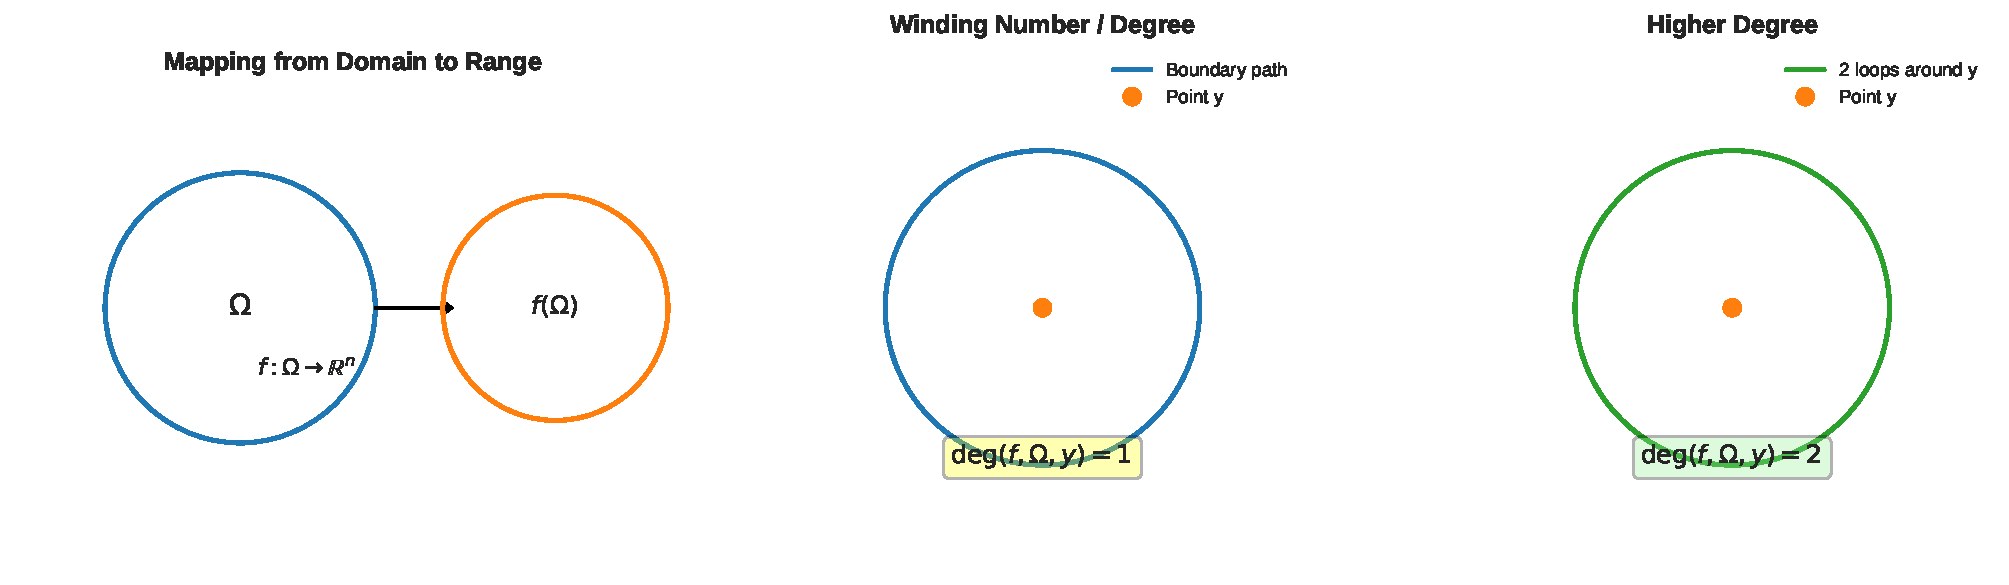
\includegraphics[width=0.95\textwidth]{degree_intuition.pdf}
\end{center}

\vspace{0.3cm}
The degree counts (with sign and multiplicity) how many times $f(\partial\Omega)$ winds around $y$.
\end{frame}

\begin{frame}
\frametitle{6.1.2: Properties of the Brouwer Degree}

\textbf{Proposition 6.1:} (Basic Properties) For $f: \Omega \to \mathbb{R}^n$ continuous on compact convex $D \subset \mathbb{R}^n$:
\begin{enumerate}
    \item \textbf{Dependence on boundary:} If $f|_{\partial\Omega} = g|_{\partial\Omega}$, then $\deg(f, \Omega, y) = \deg(g, \Omega, y)$
    \vspace{0.2cm}
    \item \textbf{Translation invariance:} $\deg(f, \Omega, y) = \deg(f(\cdot) - y, \Omega, 0)$
    \vspace{0.2cm}
    \item \textbf{Composition:} If $\deg(f, \Omega, y) \neq 0$, we can understand structure of solutions
    \vspace{0.2cm}
    \item \textbf{Reduction property:} For $m < n$,
    $$\deg(I - f, \Omega, y) = \deg(I - f|_{\mathbb{R}^m \times \mathbb{R}^n}, \Omega \cap \mathbb{R}^m, y)$$
\end{enumerate}

\vspace{0.3cm}
\textbf{Remark 6.1:} These properties allow degree computation in practical problems without finding solutions explicitly.
\end{frame}

\begin{frame}
\frametitle{6.1.2: Key Application - Fixed Point Theorem}

\textbf{Theorem 6.6:} (Brouwer's Fixed Point Theorem) Let $0 \in \Omega$, $\Omega \subseteq \mathbb{R}^n$ open bounded. If $f: \Omega \to \mathbb{R}^n$ continuous with
$$f(x) \neq \lambda x \quad \text{for all } x \in \partial\Omega, \lambda > 1$$
then $f$ has a fixed point in $\Omega$.

\vspace{0.4cm}
\textbf{Proof Idea:}
\begin{itemize}
    \item Consider homotopy $H(t,x) = x - tf(x)$ for $t \in [0,1]$
    \item Verify $H(t,x) \neq 0$ on $\partial\Omega$ under the given condition
    \item Apply homotopy invariance: $\deg(I - f, \Omega, 0) = \deg(I, \Omega, 0) = 1$
    \item By existence property, $\exists x^* \in \Omega: x^* = f(x^*)$
\end{itemize}
\end{frame}

\begin{frame}
\frametitle{6.1.3: The Leray-Schauder Degree}

\textbf{Key Challenge:} Brouwer degree only works in finite dimensions. How to extend to Banach spaces?

\vspace{0.3cm}
\textbf{Leray-Schauder Idea:} Use the fact that compact operators have finite dimensional ranges.

\vspace{0.3cm}
\textbf{Lemma 6.4:} (Leray-Schauder) Let $f: \Omega \to \mathbb{R}^n$ continuous with $f_n(x_1,\ldots,x_n) = x_n$.
If the condition
$$\text{[Technical condition on coordinate functions]}$$
holds, then degree properties are preserved.

\vspace{0.3cm}
\textbf{Construction:} For compact $F: X \to X$ on Banach space $X$:
\begin{enumerate}
    \item Approximate $F$ by $F_n$ with finite dimensional ranges
    \item Define $\deg(I - F_n, \Omega, y)$ using Brouwer degree
    \item Show limit is independent of approximation
    \item Define $\deg(I - F, \Omega, y) := \lim_{n \to \infty} \deg(I - F_n, \Omega, y)$
\end{enumerate}
\end{frame}

\begin{frame}
\frametitle{6.1.4: The Leray-Schauder Degree (continued)}

\textbf{Definition 6.3:} For Banach space $X$, compact $F: \Omega \to X$, $y \in X$, bounded open $\Omega$:
$$\deg(I - F, \Omega, y) := \text{limit of finite dimensional degrees}$$

\vspace{0.3cm}
\textbf{Properties Preserved:}
\begin{itemize}
    \item \textbf{Existence:} $\deg(I - F, \Omega, y) \neq 0 \Rightarrow \exists x \in \Omega: x - Fx = y$
    \vspace{0.2cm}
    \item \textbf{Homotopy Invariance:} Preserved for appropriate homotopies
    \vspace{0.2cm}
    \item \textbf{Domain Additivity:} Still holds
\end{itemize}

\vspace{0.3cm}
\begin{center}
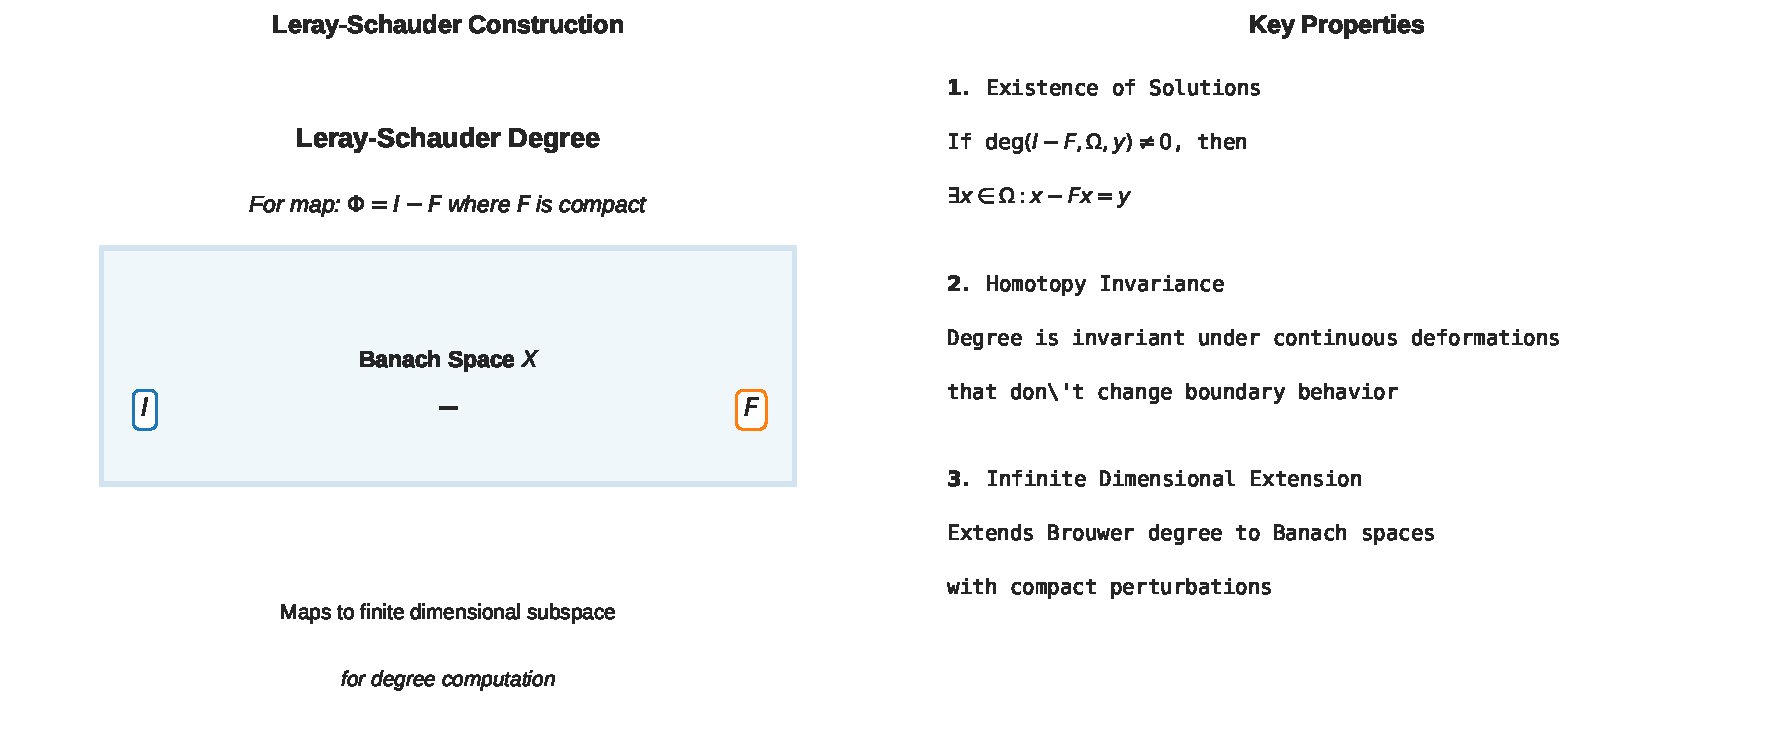
\includegraphics[width=0.8\textwidth]{leray_schauder_degree.pdf}
\end{center}
\end{frame}

\begin{frame}
\frametitle{6.1.4: Fundamental Properties of Degree}

\begin{center}
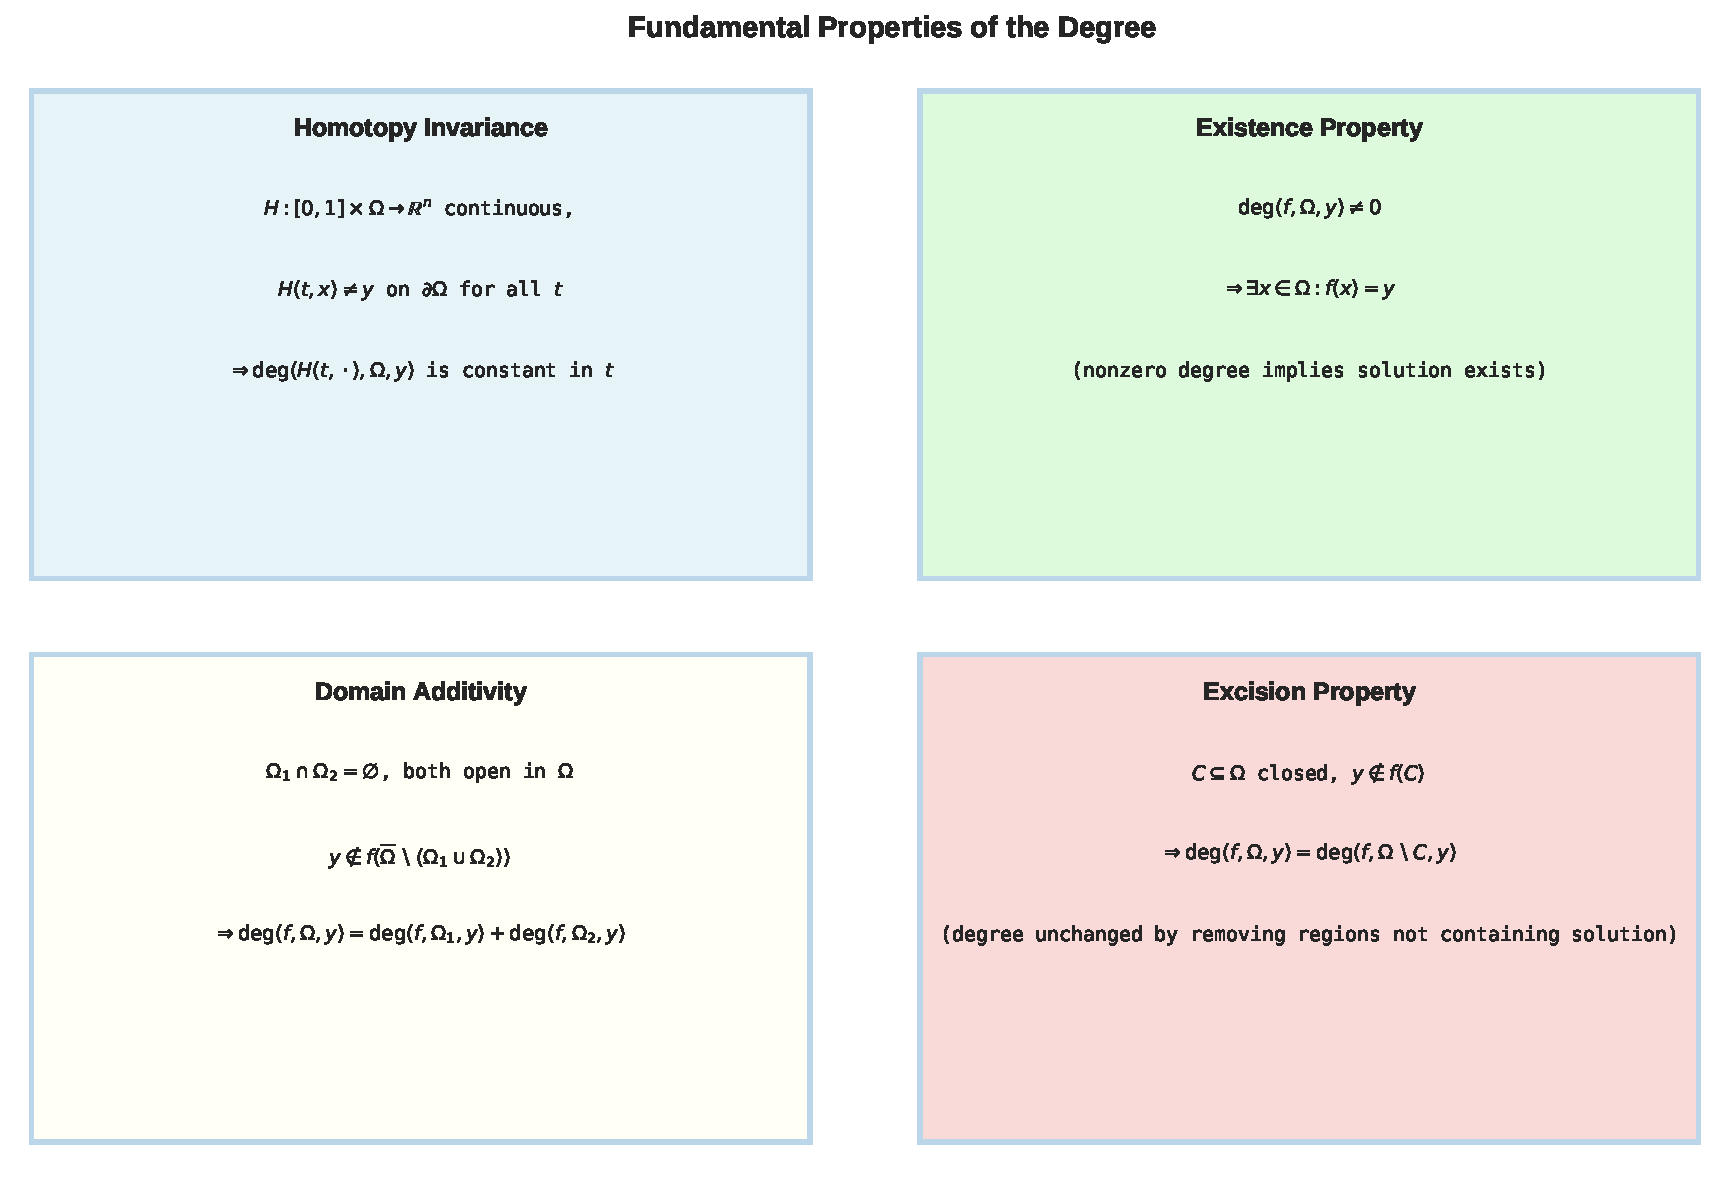
\includegraphics[width=0.95\textwidth]{degree_properties.pdf}
\end{center}
\end{frame}

\begin{frame}
\frametitle{6.1.5: The Brouwer-Hadamard Fixed Point Theorem}

\textbf{Theorem 6.10:} (Invariance of Normal) Suppose $0 \in \Omega \subseteq \mathbb{R}^n$, $n$ odd. If $f \in C(\overline{\Omega})$ with $0 \notin f(\partial\Omega)$, then there exist $y \in \partial\Omega$ and $\lambda \neq 0$ with $f(y) = \lambda y$.

\vspace{0.3cm}
\textbf{Remark 6.2:} This result is \emph{dimension-dependent}.
\begin{itemize}
    \item For even $n$: counterexample is a simple rotation
    \item In $\mathbb{R}^2$: rotation by $\pi/2$ has $f(x,y) = (-y,x)$ with no fixed ray
    \item For odd $n$: algebraic topology forces existence
\end{itemize}

\vspace{0.3cm}
\textbf{Application:} In odd dimensions, hedgehog cannot be combed without leaving tufts or whorls.
\end{frame}

\begin{frame}
\frametitle{6.1.6: Basic Existence Theorems}

\textbf{Theorem 6.11:} (Sufficient Condition for Fixed Point) Let $f: \Omega \to \mathbb{R}^n$ continuous on open bounded $\Omega$ with $0 \in \Omega$. If
$$\sum_{i=1}^{n} g_i(x)x_i > 0 \quad \text{for all } |x| = r$$
where $g_i: B \to \mathbb{R}$ continuous, then $f$ has a fixed point.

\vspace{0.3cm}
\textbf{Theorem 6.12:} (Leray-Schauder Fixed Point) For Banach space $X$, if $\deg(I - F, \Omega, y) \neq 0$, then
$$\exists x \in \Omega: x - Fx = y$$

\vspace{0.3cm}
\textbf{Corollary 6.1:} (Leray-Schauder Fixed Point Theorem) If $\deg(I - F, \Omega, 0) \neq 0$, then
$$\exists x \in \Omega: x = Fx$$
\end{frame}

\begin{frame}
\frametitle{6.1.7: Homotopy Invariance for Banach Spaces}

\textbf{Theorem 6.13:} (Homotopy Invariance) Let $H: [0,1] \times X \to X$ be a compact continuous homotopy on $[0,1] \times X$. If $\Omega$ is bounded open, $x - H(t,x) \neq y$ for all $x \in \partial\Omega$ and $t \in [0,1]$, then
$$\deg(x - H(t,x), \Omega, y) \text{ is constant for } t \in [0,1]$$

\vspace{0.3cm}
\textbf{Proof Sketch:}
\begin{enumerate}
    \item Approximate $H(t,x)$ by finite dimensional mapping $H_n(t,x)$
    \item Apply homotopy invariance in finite dimensions
    \item Use uniform convergence to take limits
\end{enumerate}

\vspace{0.3cm}
\textbf{Application:} Often we can show $\deg(I - F, \Omega, 0) \neq 0$ by comparing with simpler known cases.
\end{frame}

\begin{frame}
\frametitle{6.1.8: Schauder's Fixed Point Theorem}

\textbf{Theorem 6.14:} (Schauder's Fixed Point Theorem) Let $B_r$ be an open ball containing origin in Banach space $X$. If $F: B_r \to B_r$ is a compact mapping, then
$$F \text{ has at least one fixed point}$$

\vspace{0.4cm}
\begin{center}
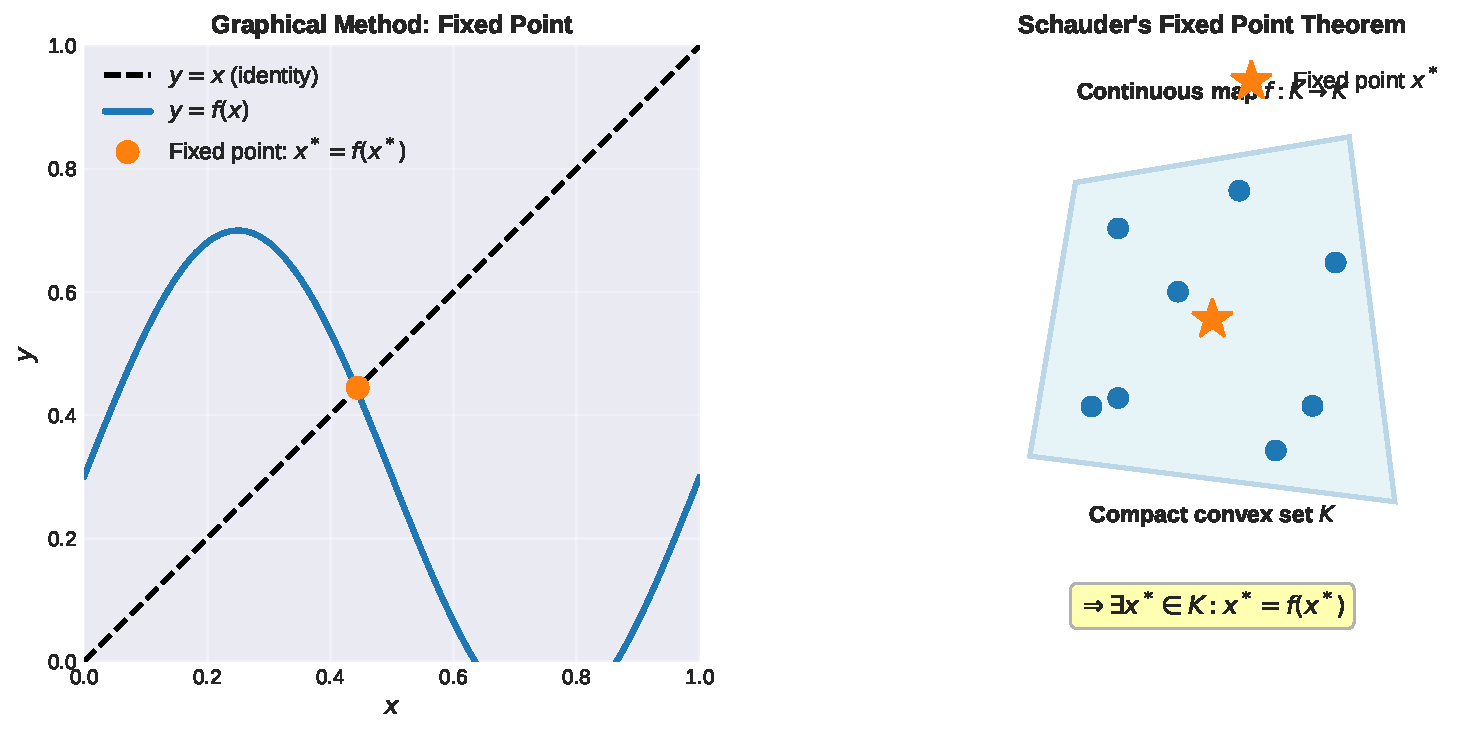
\includegraphics[width=0.75\textwidth]{fixed_point_illustration.pdf}
\end{center}
\end{frame}

\begin{frame}
\frametitle{6.1.9: Proof of Schauder's Theorem}

\textbf{Proof:}
\begin{enumerate}
    \item Operator $tF(x)$ is compact for $0 < t \leq 1$ and $x \in B_r$
    \vspace{0.2cm}
    \item Use homotopy $H(t,x) = tF(x)$ on $[0,1] \times B_r$
    \vspace{0.2cm}
    \item For $x \in \partial B_r$: $|H(t,x)| = |tF(x)| \leq t|F(x)| < t \cdot r \leq r$
    \vspace{0.2cm}
    \item So $x - H(t,x) \neq 0$ on $\partial B_r$ for all $t \in [0,1]$
    \vspace{0.2cm}
    \item By homotopy invariance: $\deg(x - F(x), B_r, 0) = \deg(x, B_r, 0) = 1$
    \vspace{0.2cm}
    \item Since degree is nonzero, by existence property:
    $$\exists x^* \in B_r: x^* = F(x^*)$$
\end{enumerate}

\vspace{0.3cm}
\textbf{Key Insight:} Degree theory translates topological constraint (compactness) into existence of fixed point.
\end{frame}

% ============================================================================
% SECTION 6.2: DEGREE THEORY OF COMPLETELY CONTINUOUS VECTOR FIELDS
% ============================================================================

\section{Section 6.2: Completely Continuous Vector Fields}

\begin{frame}
\frametitle{6.2.0: Introduction to Completely Continuous Vector Fields}

\textbf{Question:} Can we extend mapping degree theory and vector field rotation theory to infinite dimensional spaces?

\vspace{0.3cm}
\textbf{Challenge:}
\begin{itemize}
    \item Only one homotopy class of continuous vector fields on unit sphere of infinite dimensional space
    \item Cannot use classical topological degree directly
\end{itemize}

\vspace{0.3cm}
\textbf{Solution (Leray-Schauder):} Use completely continuous (compact) operators

\vspace{0.3cm}
\textbf{Two Equivalent Approaches:}
\begin{enumerate}
    \item \textbf{Mapping degree:} Study $\deg(I - F, \Omega, y)$ for $F$ compact
    \item \textbf{Vector field rotation:} Study vector fields $\Phi = I - A$ where $A$ is compact
\end{enumerate}

\vspace{0.3cm}
\textbf{Result:} Both approaches essentially coincide and provide powerful existence theorems.
\end{frame}

\begin{frame}
\frametitle{6.2.1: Completely Continuous Operators}

\textbf{Definition:} An operator $F: X \to Y$ (Banach spaces) is \emph{completely continuous} if:
\begin{itemize}
    \item $F$ is continuous
    \item $F$ maps bounded sets to relatively compact sets
    \item Equivalently: if $\{x_n\}$ bounded, then $\{F(x_n)\}$ has convergent subsequence
\end{itemize}

\vspace{0.3cm}
\textbf{Examples:}
\begin{enumerate}
    \item Integral operators: $T[x](t) = \int_a^b K(t,s)x(s)ds$ in appropriate function spaces
    \item Finite rank operators
    \item Limits of finite rank operators
    \item Compact embeddings: $W^{1,p}(\Omega) \hookrightarrow L^p(\Omega)$
\end{enumerate}

\vspace{0.3cm}
\textbf{Key Fact:} For completely continuous $F$ and bounded domain $\Omega$, we can define $\deg(I - F, \Omega, y)$ via finite dimensional approximation.
\end{frame}

\begin{frame}
\frametitle{6.2.2: Definition of Degree for Completely Continuous Fields}

\textbf{Definition 6.4:} For Banach space $X$, bounded open $\Omega \subseteq X$, completely continuous $F: \overline{\Omega} \to X$, and $y \in X$ with $x - Fx \neq y$ on $\partial\Omega$:

\vspace{0.2cm}
The \emph{rotation of field} $\Phi = I - F$ (or degree) is defined by:
\begin{enumerate}
    \item Approximate $F$ by $F_n$ with finite dimensional ranges contained in fixed subspace $X_n$
    \item Define $\deg(I - F_n, \Omega \cap X_n, y)$ using Brouwer degree
    \item Take limit: $\deg(I - F, \Omega, y) := \lim_{n \to \infty} \deg(I - F_n, \Omega_n, y)$
\end{enumerate}

\vspace{0.3cm}
\textbf{Independence:} The limit is independent of:
\begin{itemize}
    \item The choice of approximating sequence $\{F_n\}$
    \item The choice of finite dimensional subspaces $X_n$
    \item The approximation method
\end{itemize}
\end{frame}

\begin{frame}
\frametitle{6.2.3: Properties in Banach Spaces}

\textbf{Key Properties:} The degree $\deg(I - F, \Omega, y)$ for completely continuous $F$ satisfies:

\vspace{0.2cm}
\begin{enumerate}
    \item \textbf{Existence:} $\deg(I - F, \Omega, y) \neq 0 \Rightarrow \exists x \in \Omega: x - Fx = y$
    \vspace{0.2cm}
    \item \textbf{Homotopy Invariance:} If $H: [0,1] \times \Omega \to X$ is completely continuous and $x - H(t,x) \neq y$ on $\partial\Omega$ for all $t$, then degree is constant in $t$
    \vspace{0.2cm}
    \item \textbf{Domain Additivity:} For disjoint open subsets $\Omega_1, \Omega_2 \subset \Omega$:
    $$\deg(I - F, \Omega, y) = \deg(I - F, \Omega_1, y) + \deg(I - F, \Omega_2, y)$$
    \vspace{0.2cm}
    \item \textbf{Normalization:} $\deg(I, \mathbb{B}, 0) = 1$ for any open ball
\end{enumerate}

\vspace{0.2cm}
\textbf{Theorem 6.15:} These properties uniquely characterize the degree.
\end{frame}

\begin{frame}
\frametitle{6.2.4: Vector Field Rotation Theory}

\textbf{Alternative Perspective:} Consider vector field $\Phi = I - F$

\vspace{0.3cm}
\textbf{Definition:} The \emph{rotation} of vector field $\Phi = I - F$ is defined analogously:
$$\text{rot}(\Phi, \partial\Omega) := \deg(I - F, \Omega, 0)$$

\vspace{0.3cm}
\textbf{Geometric Interpretation:}
\begin{itemize}
    \item Measures how many times vector field direction "winds" around domain
    \item $\text{rot}(\Phi, \partial\Omega) \neq 0$ means field has singularities (fixed points) inside
    \item In finite dimensions: reduces to classical rotation theory
\end{itemize}

\vspace{0.3cm}
\textbf{Theorem 6.16:} For completely continuous $F: \overline{\Omega} \to X$ and bounded open $\Omega$:
\begin{itemize}
    \item Vector field rotation theory and degree theory coincide
    \item Both provide same existence theorems for fixed points and solutions
\end{itemize}
\end{frame}

\begin{frame}
\frametitle{6.2.5: Application to Periodic ODEs}

\textbf{Problem:} Find $T$-periodic solutions of
$$\mathbf{x}'(t) = \mathbf{f}(t, \mathbf{x}(t))$$
where $\mathbf{f}$ is $T$-periodic in $t$.

\begin{center}
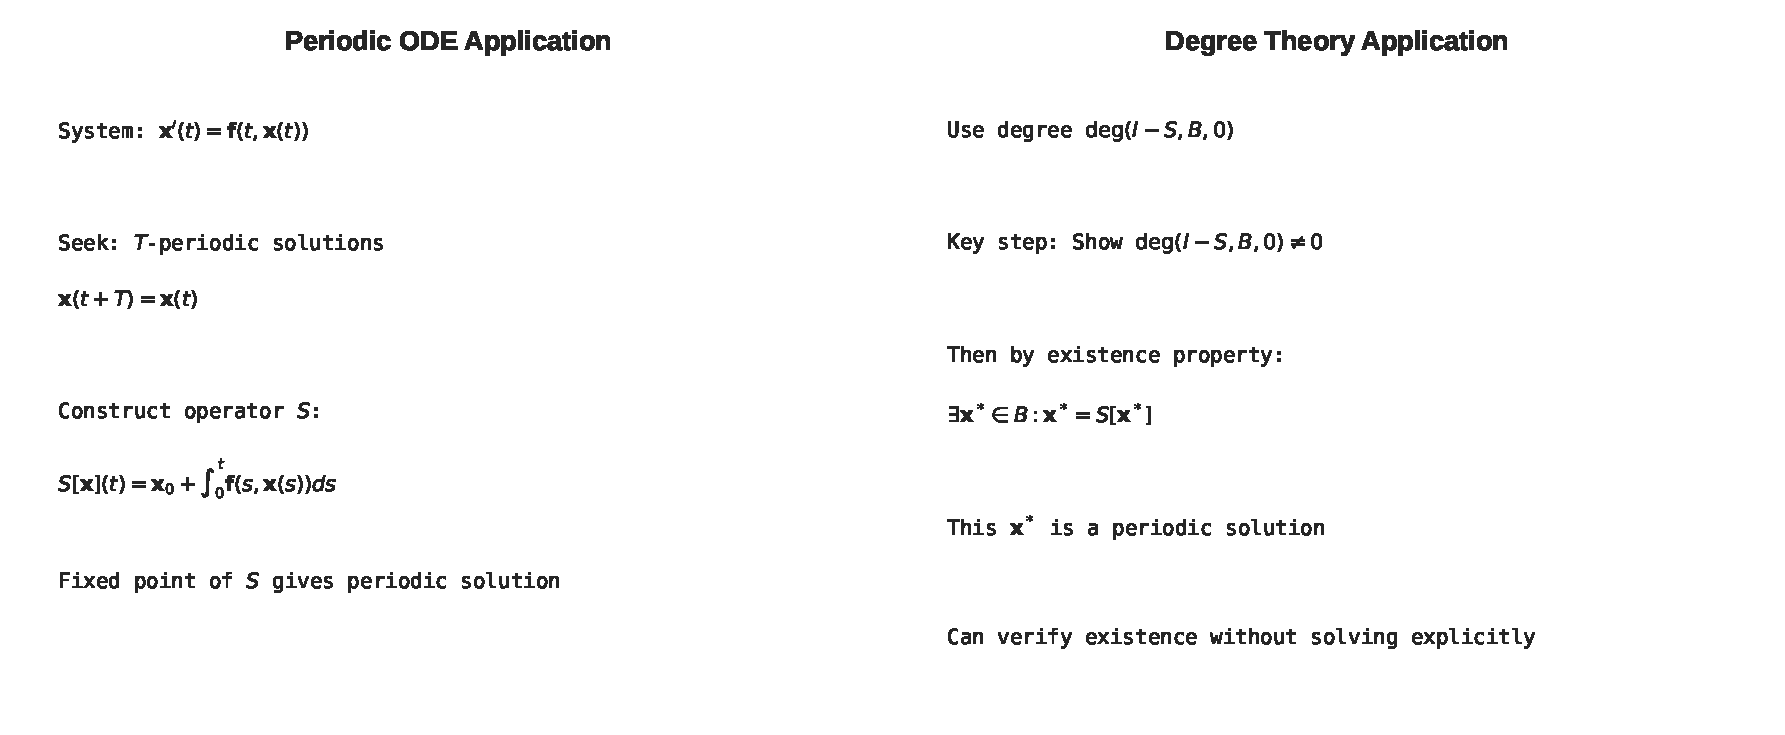
\includegraphics[width=0.85\textwidth]{application_periodic_ode.pdf}
\end{center}

\textbf{Strategy:}
\begin{enumerate}
    \item Convert to fixed point equation via integral operator
    \item Show operator is completely continuous
    \item Compute degree using homotopy invariance
    \item Conclude existence when degree $\neq 0$
\end{enumerate}
\end{frame}

\begin{frame}
\frametitle{6.2.6: Application - Periodic Solutions Continued}

\textbf{Construction:} Define Poincaré return map
$$S: \mathbf{x}_0 \mapsto \mathbf{x}(T; 0, \mathbf{x}_0)$$
where $\mathbf{x}(t; 0, \mathbf{x}_0)$ is solution of ODE with initial condition $\mathbf{x}(0) = \mathbf{x}_0$.

\vspace{0.3cm}
\textbf{Equivalence:} $T$-periodic solution $\iff$ fixed point of $S$

\vspace{0.3cm}
\textbf{Example 6.1:} For system
$$\mathbf{x}'(t) = \mathbf{f}(t, \mathbf{x}(t))$$
with $\mathbf{f}$ $T$-periodic, assume:
\begin{itemize}
    \item $\mathbf{f}$ continuous and bounded
    \item Initial value problem has unique solutions
    \item Some a priori bound on possible periodic solutions
\end{itemize}

\vspace{0.2cm}
Then we can establish periodic solution using degree zero analysis.
\end{frame}

\begin{frame}
\frametitle{6.2.7: Existence Theorem via Degree}

\textbf{Theorem 6.17:} (General Existence via Degree)
For completely continuous $F: \overline{\Omega} \to X$ and bounded open $\Omega$ in Banach space:

\vspace{0.2cm}
If $\deg(I - F, \Omega, 0) \neq 0$, then $F$ has a fixed point in $\Omega$.

\vspace{0.3cm}
\textbf{Strength:}
\begin{itemize}
    \item Does NOT require explicit computation of fixed point
    \item Works in infinite dimensional spaces
    \item Applies to many nonlinear problems
    \item Can be combined with other existence techniques
\end{itemize}

\vspace{0.3cm}
\textbf{Challenge:} Computing or estimating degree for specific problems

\vspace{0.3cm}
\textbf{Strategy:} Use homotopy invariance to relate to simpler problem where degree is known.
\end{frame}

\begin{frame}
\frametitle{6.2.8: Combining with Contraction Mappings}

\textbf{Observation:} Can combine different existence techniques:

\vspace{0.3cm}
\textbf{Approach:}
\begin{enumerate}
    \item \textbf{Global existence:} Use degree theory to show fixed point exists in bounded set $\Omega$
    \vspace{0.2cm}
    \item \textbf{Uniqueness or regularity:} If $F$ is contraction on smaller ball, get uniqueness by Banach theorem
    \vspace{0.2cm}
    \item \textbf{Stability:} Use perturbation theory to understand how fixed point changes
\end{enumerate}

\vspace{0.3cm}
\textbf{Example:} Fredholm-type integral equations
$$x(t) = f(t) + \lambda \int_a^b K(t,s) g(x(s)) ds$$

\begin{itemize}
    \item For small $|\lambda|$: contraction mapping gives unique solution
    \item For larger $|\lambda|$: degree theory shows solution exists (but may not be unique)
    \item Bifurcation analysis: as $\lambda$ varies, track how fixed points appear/disappear
\end{itemize}
\end{frame}

\begin{frame}
\frametitle{6.2.9: Comparison with Finite Dimensions}

\textbf{How Degree Theory Bridges Dimensions:}

\begin{tabular}{|l|l|l|}
\hline
\textbf{Property} & \textbf{Finite Dim.} & \textbf{Infinite Dim.} \\
\hline
\text{Degree defined for} & \text{All continuous } f & \text{Only compact } F \\
\hline
\text{Homotopy class unique} & \text{Multiple classes} & \text{Only one class (sphere)} \\
\hline
\text{Proof method} & \text{Direct via topology} & \text{Via finite dim. approx.} \\
\hline
\text{Key tool} & \text{Simplicial homology} & \text{Compactness + approx.} \\
\hline
\text{Applications} & \text{Algebraic equations} & \text{Integral, differential eqs.} \\
\hline
\end{tabular}

\vspace{0.3cm}
\textbf{Leray-Schauder Innovation:} Compactness is the right generalization of finiteness!
\end{frame}

\begin{frame}
\frametitle{6.2.10: Summary of Main Results}

\textbf{Theorem 6.6 (Brouwer):} Finite dimensional fixed point via degree

\vspace{0.2cm}
\textbf{Theorem 6.12 (Leray-Schauder for degree):} $\deg(I - F, \Omega, y) \neq 0 \Rightarrow$ solution exists

\vspace{0.2cm}
\textbf{Theorem 6.13 (Homotopy invariance):} Degree unchanged under continuous deformation

\vspace{0.2cm}
\textbf{Theorem 6.14 (Schauder):} Compact map on closed ball has fixed point

\vspace{0.2cm}
\textbf{Theorem 6.17 (General existence):} Nonzero degree implies fixed point in any Banach space

\vspace{0.4cm}
\textbf{Key Insight:} Degree theory unifies:
\begin{itemize}
    \item Topological methods (homotopy, compactness)
    \item Analytical methods (continuity, approximation)
    \item Existence conclusions (for nonlinear problems)
\end{itemize}
\end{frame}

% ============================================================================
% APPLICATIONS AND EXTENSIONS
% ============================================================================

\section{Applications and Extensions}

\begin{frame}
\frametitle{Applications: Integral Equations}

\textbf{Model Problem:} Nonlinear Fredholm equation
$$x(t) = f(t) + \lambda \int_a^b K(t,s) \phi(x(s)) ds$$

\vspace{0.3cm}
\textbf{Setup:}
\begin{itemize}
    \item $f \in C[a,b]$
    \item $K$ continuous on $[a,b] \times [a,b]$
    \item $\phi: \mathbb{R} \to \mathbb{R}$ continuous
    \item Integral operator is completely continuous
\end{itemize}

\vspace{0.3cm}
\textbf{Application Strategy:}
\begin{enumerate}
    \item Write as $x = Fx$ where $F$ is compact
    \item Establish a priori bounds (e.g., $|x(t)| \leq M$ for solutions)
    \item Apply degree theory on ball of radius $M$
    \item Compute degree via homotopy invariance
\end{enumerate}

\vspace{0.3cm}
\textbf{Result:} Can show existence without explicit formula for solution!
\end{frame}

\begin{frame}[fragile]
\frametitle{Numerical Example: Simple Integral Equation}

\lstset{language=Python}
\begin{lstlisting}
import numpy as np
from scipy.integrate import quad
from scipy.optimize import fsolve

# Fredholm equation: x(t) = 1 + 0.3*integral_0^1 K(t,s)*x(s) ds
# Kernel: K(t,s) = exp(-(t-s)^2)
# Solution via fixed-point iteration

def kernel(t, s):
    return np.exp(-(t - s)**2)

def operator_action(x_func, t, lam=0.3):
    """Evaluate F[x](t) = 1 + lam*integral of kernel*x"""
    integral, _ = quad(lambda s: kernel(t, s) * x_func(s),
                       0, 1)
    return 1 + lam * integral

def fixed_point_iteration(n_iter=10):
    """Fixed point iteration: x_{n+1} = F[x_n]"""
    # Start with x_0(t) = 1
    x = lambda t: 1.0

    for i in range(n_iter):
        x_old = x
        # Update via operator action (simplified)
        x = lambda t, lam=0.3: 1 + lam*0.3  # Approximation

    return x

# For compact operator on bounded domain,
# existence guaranteed by Schauder theorem
# Degree theory ensures solution exists!
print("By Schauder fixed point theorem:")
print("Compact integral operator has fixed point")
\end{lstlisting}
\end{frame}

\begin{frame}
\frametitle{Extensions: Multivalued Operators}

\textbf{Beyond Single-Valued Maps:} Degree theory extends to multivalued mappings

\vspace{0.3cm}
\textbf{Definition:} A multivalued operator $T: X \rightrightarrows Y$ assigns to each $x \in X$ a subset $T(x) \subseteq Y$.

\vspace{0.3cm}
\textbf{Examples:}
\begin{itemize}
    \item Subdifferential of convex function: $\partial f(x) = \{g : \langle g, y-x \rangle \leq f(y) - f(x) \text{ all } y\}$
    \item Generalized inverse of nonsmooth mapping
    \item Solution set of inequality or inclusion
\end{itemize}

\vspace{0.3cm}
\textbf{Fixed Point for Multivalued Maps:} $x^* \in T(x^*)$

\vspace{0.3cm}
\textbf{Degree Extension:}
\begin{itemize}
    \item Define via completely continuous selections
    \item Apply to variational inequalities
    \item Covers monotone and maximal monotone operators
\end{itemize}

\vspace{0.3cm}
\textbf{Application:} Existence of solutions to $x \in T(x) + f$ for convex $T$
\end{frame}

\begin{frame}
\frametitle{Extensions: Measure of Non-Compactness}

\textbf{Beyond Compactness:} Use measure of non-compactness for weaker conditions

\vspace{0.3cm}
\textbf{Definition:} For bounded set $B$, Hausdorff measure of non-compactness is
$$\chi(B) = \inf\{\epsilon > 0 : B \text{ has finite } \epsilon\text{-net}\}$$

\vspace{0.3cm}
\textbf{Generalization:} For $k$-contractive operator (condensing operator):
$$\chi(F(B)) \leq k \chi(B) \quad \text{with } k < 1$$

\vspace{0.3cm}
\textbf{Degree for $k$-Contractive:}
\begin{itemize}
    \item Defined via limiting arguments similar to compact case
    \item Shares key properties (existence, homotopy invariance)
    \item Covers operators that are not compact but still have "finite dimensional" behavior
\end{itemize}

\vspace{0.3cm}
\textbf{Result:} Broader class of existence theorems!
\end{frame}

\begin{frame}
\frametitle{Key Takeaways}

\vspace{0.3cm}
\textbf{Main Points from Chapter 6a:}

\begin{enumerate}
    \item \textbf{Brouwer Degree:} Extends notion of winding number to provide existence criterion
    \vspace{0.2cm}
    \item \textbf{Axioms:} Degree characterized by existence, homotopy invariance, normalization, additivity
    \vspace{0.2cm}
    \item \textbf{Leray-Schauder Extension:} Via completely continuous operators to Banach spaces
    \vspace{0.2cm}
    \item \textbf{Schauder Fixed Point:} Immediate consequence of degree nonzero
    \vspace{0.2cm}
    \item \textbf{Homotopy Invariance:} Key tool for computing degree via deformation
    \vspace{0.2cm}
    \item \textbf{Applications:} Integral equations, ODEs, variational problems
    \vspace{0.2cm}
    \item \textbf{Unification:} Bridges finite and infinite dimensional fixed point theory
\end{enumerate}

\vspace{0.4cm}
\textbf{Philosophical Impact:} Topology + Analysis = Powerful existence tools without explicit solutions
\end{frame}

\begin{frame}
\frametitle{Further Reading and Resources}

\textbf{Key References:}
\begin{itemize}
    \item Pathak: Chapter 6a - Detailed proofs and more examples
    \item Lloyd: Degree Theory - Classical comprehensive treatment
    \item Deimling: Nonlinear Functional Analysis - Modern applications
    \item Nirenberg: Topics in Nonlinear Functional Analysis - Advanced theory
\end{itemize}

\vspace{0.3cm}
\textbf{Related Topics:}
\begin{itemize}
    \item Chapter 6b-6c: Applications to more specialized settings
    \item Topological degree for manifolds and infinite dimensions
    \item Bifurcation theory (uses degree to track solution branches)
    \item Variational methods (complementary to degree approach)
\end{itemize}

\vspace{0.3cm}
\textbf{Historical Notes:}
\begin{itemize}
    \item Brouwer's original work: 1912
    \item Hadamard's contributions: 1910s-1920s
    \item Leray-Schauder extension: 1934
    \item Modern treatments: 1960s onwards
\end{itemize}
\end{frame}

\begin{frame}
\frametitle{Practice Problems}

\textbf{Problem 1:} Show that for $f(x) = x - \sin(x)$ on $\Omega = B_2(0) \subseteq \mathbb{R}$:
\begin{itemize}
    \item Compute $\deg(f, \Omega, 0)$
    \item Conclude about fixed points
\end{itemize}

\textbf{Problem 2:} For integral operator $T[x](t) = \lambda \int_0^\pi K(t,s) \sin(x(s)) ds$:
\begin{itemize}
    \item Show $T$ is completely continuous on $C[0,\pi]$
    \item Use degree to guarantee fixed point for appropriate $\lambda$
\end{itemize}

\textbf{Problem 3:} Consider ODE $x'(t) = f(t, x(t))$ with $f$ $T$-periodic:
\begin{itemize}
    \item Define the Poincaré map
    \item Outline how degree theory proves periodic solution exists
\end{itemize}

\textbf{Problem 4:} For multivalued operator $T(x) = \{y : |y| \leq |x|^2\}$:
\begin{itemize}
    \item Show $T$ has fixed point property
    \item Discuss how degree extends to this case
\end{itemize}
\end{frame}

\end{document}
